\section{Introduction to Machine Learning}


Machine Learning: Field of study that gives computers the ability to learn without being explicitly programmed. \\

Well-posed Learning Problem: A computer program is said to learn from experience E with respect to some task T and some performance measure P, if its performance on T, as measured by P, improves with experience E. \\

Machine Learning Algorithms
\begin{itemize}
\item Supervised Learning
\item Unsupervised Learning
\item Reinforcement Learning
\item Recommender Systems
\end{itemize}


\subsection{Supervised Learning}

In supervised learning, we are given a data set and already know what our correct output should look like, having the idea that there is a relationship between the input and the output.\\

Supervised learning problems are categorized into "regression" and "classification" problems. In a regression problem, we are trying to predict results within a continuous output, meaning that we are trying to map input variables to some continuous function. In a classification problem, we are instead trying to predict results in a discrete output. In other words, we are trying to map input variables into discrete categories. \\

In \textbf{supervised learning}, the "right answers" are known.\\

A \textbf{Regression} is predicting a value! For example Given a picture of a person, we have to predict their age on the basis of the given picture\\

A \textbf{classification} is breaking into groups or discrete values.  For example Given a patient with a tumor, we have to predict whether the tumor is malignant or benign.\\


\subsection{Unsupervised Learning}

In \textbf{unsupervised learning}, the "right answers" are \textbf{not} known.\\



Unsupervised learning allows us to approach problems with little or no idea what our results should look like. We can derive structure from data where we don't necessarily know the effect of the variables.\\

We can derive this structure by clustering the data based on relationships among the variables in the data.\\

With unsupervised learning there is no feedback based on the prediction results. \\

\subsection{Model}

Input variables or input features are denoted as $x^{(i)}$\\
Output or target variable we are trying to predict are denoted as $y^{(i)}$\\
The pair $(x^{(i)}, y^{(i)})$ is called a training example.\\

To establish notation for future use, we’ll use $x^{(i)}$ to denote the \textbf{“input”} variables (living area in this example), also called input features, and $y^{(i)}$ to denote the \textbf{“output”} or target variable that we are trying to predict (price). A pair $(x^{(i)}, y^{(i)})$ is called a \textbf{training example}, and the dataset that we’ll be using to learn—a list of m training examples $(x^{(i)}, y^{(i)})$; i=1,...,m—is called a \textbf{training set}. Note that the superscript “(i)” in the notation is simply an index into the training set, and has nothing to do with exponentiation. We will also use \textbf{X} to denote the space of input values, and \textbf{Y} to denote the space of output values. In this example, X = Y = $\mathbb{R}$.

To describe the supervised learning problem slightly more formally, our goal is, given a training set, to learn a function
\begin{equation}
  h : X \rightarrow Y
\end{equation}
so that h(x) is a “good” predictor for the corresponding value of y. For historical reasons, this function h is called a hypothesis. Seen pictorially, the process is therefore like this:

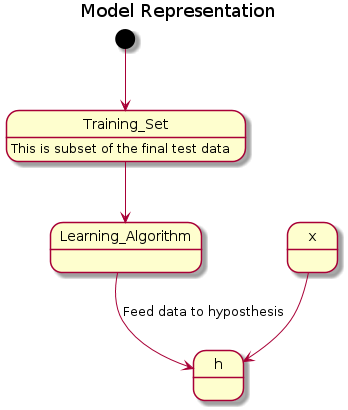
\includegraphics{model_representation.png}

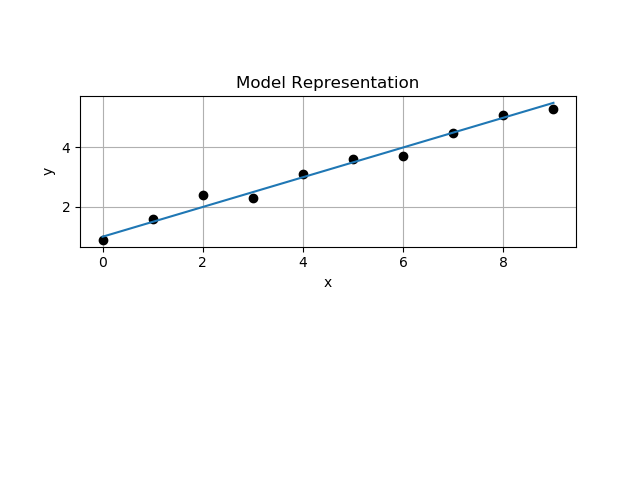
\includegraphics{python/model_plot_representation.png}\\

This is an attempt at a linear fit for this data.  It is not quite a match, but it is very close.  The plot for the line is $y=0.5x+1$ which is our hypothesis fuction h. 


\subsection{Cost Functions}

We can measure the accuracy of our hypothesis function by using a \textbf{cost function}. This takes an average difference (actually a fancier version of an average) of all the results of the hypothesis with inputs from x's and the actual output y's. \\

\begin{equation}
J(\theta_{0}, \theta_{1}) = \frac{1}{2m} \sum_{i=1}^{m} (\hat{y} -y^{i})^{2} = \frac{1}{2m} \sum_{i=1}^{m} (h_{\theta}(x^{i})-y^{i})^2
\end{equation}

m is the number of training examples. The goal is to minimize $J(\theta_{0}, \theta_{1})$.

To break it apart, it is $\frac{1}{2} \bar{x}$ where $\bar{x}$ is the mean of the squares of $h_{\theta}(x^{i}) -y^{i}$, or the difference between the predicted value and the actual value.\\

This function is otherwise called the \textbf{Squared error function}, or \textbf{Mean squared error}. The mean is halved $\frac{1}{2}$ as a convenience for the computation of the gradient descent, as the derivative term of the square function will cancel out the $\frac{1}{2}$ term. \\

For our previous example of $y=0.5x + 1$, we have $h_{\theta}(x^{i}) = \theta_{0} + \theta_{1}x^{i}$.  This leads to our cost function of 

\begin{equation}
J(\theta_{0}, \theta_{1}) = \frac{1}{2m} \sum_{i=1}^{m} (\theta_{0} + \theta_{1}x^{i} - y^{i})^{2} 
\end{equation}

Choose $\theta_{0}, \theta_{1}$ so that $h_{\theta}(x)$ is close to $y$ for training examples $(x,y)$\\
